\documentclass[tikz, convert = false]{standalone}

\usepackage[utf8]{inputenx}%  http://ctan.org/pkg/inputenx
% Euler for math | Palatino for rm | Helvetica for ss | Courier for tt
\renewcommand{\rmdefault}{ppl}% rm
\linespread{1.05}% Palatino needs more leading
\usepackage[scaled]{helvet}% ss //  http://ctan.org/pkg/helvet
\usepackage{courier}% tt // http://ctan.org/pkg/courier
\usepackage{eulervm}  %  http://ctan.org/pkg/eulervm
% a better implementation of the euler package (not in gwTeX)
\normalfont%
\usepackage[T1]{fontenc}%  http://ctan.org/pkg/fontenc
\usepackage{textcomp}%  http://ctan.org/pkg/textcomp

\usetikzlibrary{calc}
\usetikzlibrary{intersections}

\begin{document}
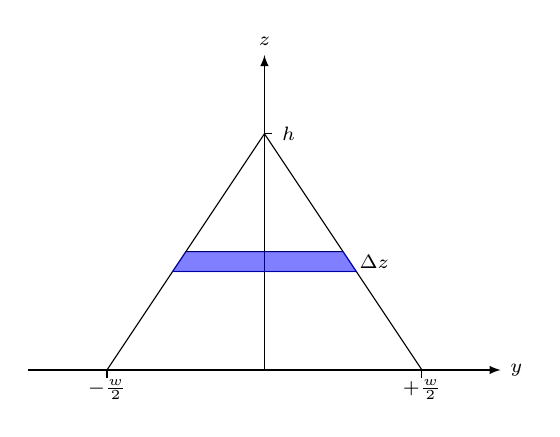
\begin{tikzpicture}
  \coordinate (h) at (0, 3);
  \coordinate (O) at (0, 0);

  \draw (O) -- +(-3, 0);
  \draw[-latex] (O) -- +(3, 0) node[right, font = \scriptsize] {$y$};
  \draw[-latex] (O) -- +(0, 4) node[above, font = \scriptsize] {$z$};

  \foreach \x/\s in {-2/{-}, 2/{+}}{
    \draw (\x, 0) coordinate (w\s) -- +(0, -0.1) node[below,
    font = \scriptsize] at (\x, 0) {$\s\frac{w}{2}$};
  }

  \draw[name path = uslope] (w-.center) -- (h);
  \draw[name path = dslope] (w+.center) -- (h);

  \path[name path = uline] (-3, 1.5) -- (3, 1.5);
  \path[name path = dline] (-3, 1.25) -- (3, 1.25);

  \path[name intersections = {of = uline and uslope, by = P1}];
  \path[name intersections = {of = uline and dslope, by = P2}];
  \path[name intersections = {of = dline and uslope, by = P3}];
  \path[name intersections = {of = dline and dslope, by = P4}];

  \draw (P1) -- (P2);
  \draw (P3) -- (P4);

  \filldraw[opacity = .5, blue] (P1) -- (P2) -- (P4) -- (P3) -- cycle;

  \path (P2) -- (P4) node[right, pos = .5, font = \scriptsize] {$\Delta z$};

  \draw (h) -- +(0.1, 0) node[right, font = \scriptsize] {$h$};
\end{tikzpicture} 
\end{document}